%%%%%%%%%%%%%%%%%%%%%%%%%%%%%%%%%%%%%%%%%%%%%%%%%%%%%%%%%%%%%%%%%%%%%%%%%%%%
% AGUJournalTemplate.tex: this template file is for articles formatted with LaTeX
%
% This file includes commands and instructions
% given in the order necessary to produce a final output that will
% satisfy AGU requirements, including customized APA reference formatting.
%
% You may copy this file and give it your
% article name, and enter your text.
%
%
% Step 1: Set the \documentclass
%
% There are two options for article format:
%
% PLEASE USE THE DRAFT OPTION TO SUBMIT YOUR PAPERS.
% The draft option produces double spaced output.
%

%% To submit your paper:
\documentclass[draft]{agujournal2019}
\usepackage{url} %this package should fix any errors with URLs in refs.
\usepackage{lineno}
\linenumbers
%%%%%%%
% As of 2018 we recommend use of the TrackChanges package to mark revisions.
% The trackchanges package adds five new LaTeX commands:
%
%  \note[editor]{The note}
%  \annote[editor]{Text to annotate}{The note}
%  \add[editor]{Text to add}
%  \remove[editor]{Text to remove}
%  \change[editor]{Text to remove}{Text to add}
%
% complete documentation is here: http://trackchanges.sourceforge.net/
%%%%%%%

\draftfalse

%% Enter journal name below.
%% Choose from this list of Journals:
%
% JGR: Atmospheres
% JGR: Biogeosciences
% JGR: Earth Surface
% JGR: Oceans
% JGR: Planets
% JGR: Solid Earth
% JGR: Space Physics
% Global Biogeochemical Cycles
% Geophysical Research Letters
% Paleoceanography and Paleoclimatology
% Radio Science
% Reviews of Geophysics
% Tectonics
% Space Weather
% Water Resources Research
% Geochemistry, Geophysics, Geosystems
% Journal of Advances in Modeling Earth Systems (JAMES)
% Earth's Future
% Earth and Space Science
% Geohealth
%
% ie, \journalname{Water Resources Research}

\journalname{Geophysical Research Letters}


\begin{document}

%% ------------------------------------------------------------------------ %%
%  Title
%
% (A title should be specific, informative, and brief. Use
% abbreviations only if they are defined in the abstract. Titles that
% start with general keywords then specific terms are optimized in
% searches)
%
%% ------------------------------------------------------------------------ %%

% Example: \title{This is a test title}

\title{Depth of the source of the tectonic tremor in the northeastern Olympic Peninsula, Washington}

%% ------------------------------------------------------------------------ %%
%
%  AUTHORS AND AFFILIATIONS
%
%% ------------------------------------------------------------------------ %%

% Authors are individuals who have significantly contributed to the
% research and preparation of the article. Group authors are allowed, if
% each author in the group is separately identified in an appendix.)

% List authors by first name or initial followed by last name and
% separated by commas. Use \affil{} to number affiliations, and
% \thanks{} for author notes.
% Additional author notes should be indicated with \thanks{} (for
% example, for current addresses).

% Example: \authors{A. B. Author\affil{1}\thanks{Current address, Antartica}, B. C. Author\affil{2,3}, and D. E.
% Author\affil{3,4}\thanks{Also funded by Monsanto.}}

\authors{Ariane Ducellier\affil{1}}


% \affiliation{1}{First Affiliation}
% \affiliation{2}{Second Affiliation}
% \affiliation{3}{Third Affiliation}
% \affiliation{4}{Fourth Affiliation}

\affiliation{1}{University of Washington}
%(repeat as many times as is necessary)

%% Corresponding Author:
% Corresponding author mailing address and e-mail address:

% (include name and email addresses of the corresponding author.  More
% than one corresponding author is allowed in this LaTeX file and for
% publication; but only one corresponding author is allowed in our
% editorial system.)

% Example: \correspondingauthor{First and Last Name}{email@address.edu}

\correspondingauthor{Ariane Ducellier}{ducela@uw.edu}

%% Keypoints, final entry on title page.

%  List up to three key points (at least one is required)
%  Key Points summarize the main points and conclusions of the article
%  Each must be 100 characters or less with no special characters or punctuation and must be complete sentences

% Example:
% \begin{keypoints}
% \item	List up to three key points (at least one is required)
% \item	Key Points summarize the main points and conclusions of the article
% \item	Each must be 100 characters or less with no special characters or punctuation and must be complete sentences
% \end{keypoints}

\begin{keypoints}
\item enter point 1 here
\item enter point 2 here
\item enter point 3 here
\end{keypoints}

%% ------------------------------------------------------------------------ %%
%
%  ABSTRACT
%
% A good abstract will begin with a short description of the problem
% being addressed, briefly describe the new data or analyses, then
% briefly states the main conclusion(s) and how they are supported and
% uncertainties.
%% ------------------------------------------------------------------------ %%

%% \begin{abstract} starts the second page

\begin{abstract}
enter abstract here

\end{abstract}



%% ------------------------------------------------------------------------ %%
%
%  TEXT
%
%% ------------------------------------------------------------------------ %%

%%% Suggested section heads:
% \section{Introduction}
%
% The main text should start with an introduction. Except for short
% manuscripts (such as comments and replies), the text should be divided
% into sections, each with its own heading.

% Headings should be sentence fragments and do not begin with a
% lowercase letter or number. Examples of good headings are:

% \section{Materials and Methods}
% Here is text on Materials and Methods.
%
% \subsection{A descriptive heading about methods}
% More about Methods.
%
% \section{Data} (Or section title might be a descriptive heading about data)
%
% \section{Results} (Or section title might be a descriptive heading about the
% results)
%
% \section{Conclusions}


\section{Introduction}
%Text here ===>>>

Tremor is a long (several seconds to many minutes), low amplitude seismic signal, with emergent onsets, and an absence of clear impulsive phases. Tectonic tremor have been explained as a swarm of small, low frequency earthquakes (LFEs) ~\cite{SHE_2007_nature}, that is small magnitude earthquakes (M $\sim$ 1) which frequency content (1-10 Hz) is lower than for ordinary earthquakes (up to 20 Hz). The source of the LFEs is located on the plate boundary, and their focal mechanisms represent shear slip on a low-angle thrust fault dipping in the same direction as the plate interface ~\cite{IDE_2007_GRL}. Due to the lack of clear impulsive phases in the tremor signal, it is difficult to determine the depth of the tremor source with the same precision, and it is assumed to be also located close to the plate boundary. In subduction zones such as Nankai and Cascadia, tectonic tremor observations are spatially and temporally correlated with slow slip observations ~\cite{OBA_2002,ROG_2003}. Due to this correlation, these paired phenomena have been called Episodic Tremor and Slip (ETS). \\

The occurrence of tremor seems to be linked to low effective normal stress or high fluid pressure near the location of the source of the tremor. Indeed, ~\citeA{SHE_2006} have observed a high ratio between P-wave velocity and S-wave velocity in the subducting oceanic crust near the location of the LFEs in western Shikoku, Japan. They hypothesized that the source of the fluids is the dehydration of hydrous minerals within the subducting oceanic crust. In Cascadia, ~\citeA{AUD_2009} have computed receiver functions of teleseismic waves in Vancouver Island, and analyzed the delay times between the forward-scattered P-to-S, and back-scattered P-to-S and S-to-S conversions at two seismic reflectors identified as the top and bottom of the oceanic crust. It allowed them to compute the P-to-S velocity ratio of the layer and the S-wave velocity contrast at both interfaces. The very low Poisson's ratio of the layer could not be explained by the mineral composition, and they interpreted it as evidence for high pore-fluid pressure. They explained the sharp velocity contrast on top of the layer as a low permeability boundary between the oceanic plate and the overriding continental crust. They hypothesized that the low permeability of the plate interface may be due either to grain-size reduction or to the precipitation of minerals from migrating fluids. At greater depth, the large volume reduction and water release accompanying eclogitization in the subducted oceanic crust, and the large volume expansion accompanying serpentinization in the mantle wedge, could increase the permeability of the plate boundary through fracture generation. A possible cause of ETS events could be periodic cycles of steady pore-fluid pressure build-up from dehydration of subducted oceanic crust, fluid release from fracturing of the interface during ETS, and subsequent precipitation sealing of the plate boundary. \\

Moreover, the variations of tremor occurrence have been linked to tidal cycles. ~\citeA{NAK_2008} noticed that tremor swarms often exhibit occurrences with a periodicity of about 12 or 24 h, and concluded that they are probably related to Earth tides. Their occurrence is also well correlated with time evolution of Coulomb failure stress (CFS) and CFS rate. However, they noted that tremor occurrences are advanced by a few hours relative to CFS, from which they conclude that a simple Coulomb threshold model is not sufficient to explain tremor occurrence. Instead they point out that the correlation of tremor occurrence and the CFS rate as well as the time delay between both could be reproduced by using the rate- and state-dependent friction law. ~\citeA{THO_2009} have also observed that tremor occurrence on the deep San Andreas fault are correlated with small, tidal shear stress changes. They explain it by a very weak fault zone with low effective normal stress, probably due to near-lithostatic pore pressures at the depth of the tremor source region. \\

~\citeA{SHE_2006} made two hypothesis explaining how highly pressured fluids could generate tectonic tremor. A first possibility is that tremor is generated by the movement of fluids at depth, either by hydraulic fracturing or by coupling between the rock and fluid flow. The accompanying slip could be triggered by the same fluid movement that generates the tremor or, alternatively, the fluid flow could be a response to changes in stress and strain induced by the accompanying slip. The second possibility is that tremor is generated by slow otherwise aseismic shear slip on the plate interface as slip locally accelerates owing to the effects of geometric or physical irregularities on the plate interface. Fluids would then play an auxiliary role, altering the conditions on the plate interface to enable transient slip events, without generating seismic waves directly. \\

~\citeA{FAG_2011} have explained why the generation of tectonic tremor is restricted to a small range of depth along the plate boundary by computing the equilibrium mineral assemblages at different P-T conditions, and comparing it to the P-T path of the subducting oceanic crust in Shikoku and Cascadia. They noted that for most of the P-T path, there are no dehydration reactions and the slab remains fluid-absent, except for depths between 30 and 35 km depth for Shikoku, and depths between 30 and 40 km for Cascadia, where the mineral model predicts significant water release. These depth ranges coincide with the depth range where tremor has been observed. They concluded that abundant tremor activity requires metamorphic conditions where localized dehydration occurs during subduction, and that subduction zones where dehydration reactions are more widely distributed will produce a more diffuse pattern of tremor activity that would be harder to detect. \\

Moreover, the generation of slow slip and tectonic tremor has been related to the presence of quartz in the overriding continental crust. Indeed, ~\citeA{AUD_2014} studied the relationship between the ratio between P-wave velocity and S-wave velocity in the subducted oceanic crust and the forearc and the periodicity of slow earthquakes. They computed the $V_P / V_S$ ratio from receiver functions and data from the literature. They noticed that slow earthquakes are associated with a high $V_P / V_S$ ratio in the subducted oceanic crust, but without relationship with recurrence time. However, they pointed out that the recurrence time of slow earthquakes increases linearly with the $V_P / V_S$ ratio of the forearc. Moreover, along a margin-perpendicular profile from northern Cascadia, the $V_P / V_S$ ratio of the forearc, and the recurrence time of Episodic Tremor and Slip (ETS) events, decrease with increasing depth. The authors explained the low $V_P / V_S$ ratio in the forearc by the enrichment of forearc minerals in fluid-dissolved silica derived from the dehydration of the downgoing slab. However, they estimated that the fluid flux required for the formation of quartz veins was two orders of magnitude greater than the fluid production rates estimated from the dehydration of the slab. They hypothesized that silica-saturated fluids may originate from the complete serpentinization of the mantle near the wedge corner. They suggested that higher temperature and quartz content at depth may lead to faster dissolution - precipitation processes and more frequent slip events. Their model could also explain the global variation in recurrence time, with mafic silica-poor regions having longer ETS recurrence times that felsic silica-rich regions. \\

~\citeA{HYN_2015} have also investigated the processes that control the ETS in the Cascadia subduction zone. They noticed that the high temperatures in the young subducting oceanic plate, the geodetic data, and the recordings of coseismic subsidence in buried coastal marshes during past great earthquakes, all point out to a downdip limit of the seismogenic zone located offshore. The position of the slow slip and the tremor is well known, although the depths have some uncertainty. The slip may extend seaward of the tremor, but there is a clear separation between the seismogenic zone and the ETS zone, with the ETS zone being located about 70 km east of the downdip limit of the seismogenic zone, and the volcanic arc being located about 100 km east of the ETS zone. A previous study showed that the position of the subduction zone ETS does not coincide with a specific temperature or dehydration reaction. The authors pointed out that ETS has been related to high pore fluid pressures close to the plate boundary. They argued that the bending of the subducting plate at the ocean trench may introduce a large amount of water in the upper oceanic mantle, resulting in extensive serpentinization. Moreover, the serpentinization of the fore-arc mantle corner may increase its vertical impermeability, while keeping a high permeability parallel to the fault, thus channelling all the fluid updip in the subducting oceanic crust. The dehydration of the serpentinite from the upper oceanic mantle, and the focusing of rising fluids along the plate boundary should result in large amounts of fluids available at the fore-arc mantle corner. Additionally, there seems to be a good coincidence between the location of the fore-arc mantle corner, and the location of ETS. The authors then observed that the deep fore-arc crust has a very low Poisson's ratio (less than 0.22), and that the only mineral with a very low Poisson's ratio is quartz (about 0.1), which led them to conclude that there may be a significant amount of quartz (about 10 \% in volume) in the deep fore-arc crust above the fore-arc mantle. Moreover, as the solubility of silica increases with temperature, fluids generated at depth and rising up the subduction channel should be rich in silica. The authors concluded that there may be a relation between quartz veins formation in the deep fore-arc crust and ETS. However, several constraints as the magnitude and mechanism of the LFEs, and the vertical extent of the tremor should be explained. \\

Quartz veins have indeed been observed in exhumed subduction zone. For instance, ~\citeA{FAG_2014} have studied an exhumed shear zone representing the subduction megathrust before its incorporation into the accretionary prism. They focused their study on a 30 m high by 80 m long cliff exposure where foliation has developed as a result of shearing along the subduction thrust interface. They identified two groups of quartz veins, foliation-parallel veins, and discordant veins, that must have formed for an extended time before, during, and after foliation development. They interpret the foliation-parallel veins as having been formed by viscous shear flow, and note that the shear stain rate due to the flow may be high enough to accommodate a slow slip strain rate of $\sim 10^{-9} s{-1}$, for a typical subduction thrust thickness of 30 m ~\cite{ROW_2013}. They interpret the discordant veins as having been formed by brittle deformation caused by locally elevated fluid pressure. The size of the structures where brittle deformation is observed (meters to hundreds of meters) is compatible with the size of the asperity rupturing during an LFE. Tremor and slow slip may thus be a manifestation of brittle-viscous deformation in the shear zone. \\

However, the zone with high low Poisson's ratio observed by ~\citeA{HYN_2015} has a large vertical extent (about 10 kilometers). If the whole zone is associated with quartz deposition and tectonic tremor generation, we should also observe a large vertical distribution of the source of the tremor. ~\citeA{KAO_2006}) have used a Source Source Scanning Algorithm to detect and locate tremor, and have indeed located tremor in the continental crust, with a wide depth range of over 40 km. They noted that this wide depth range could not arise from either analysis uncertainties or a systematic bias in the velocity model they used. A follow-up study by ~\citeA{KAO_2009}) gave a thickness of the tremor zone of 5-10 km. This depth range is inconsistent with the depth of the LFEs, which have been located on a thin band at or near the plate interface with a rupture mechanism that corresponds to the thrust dip angle ~\cite{IDE_2007_GRL}. Further study is thus needed to narrow the uncertainty on the depth of the source of the tremor, and verify whether tremor could occur in a wider zone than LFEs. \\

Several methods have been developed to detect and locate tectonic tremor or LFEs using the cross correlation of seismic signals. The main idea is to find similar waveforms in two different seismic signals, which could correspond to a single tremor or LFE recorded at two different stations, or two different tremors or LFEs with the same source location but occurring at two different times and recorded by the same station. A first method consists in comparing the envelopes of seismograms at different stations ~\cite{OBA_2002,WEC_2008}, or directly the seismograms at different stations ~\cite{RUB_2013}. For instance, ~\citeA{WEC_2008} computed the cross correlations of envelope seismograms for a set of 20 stations in western Washington and southern Vancouver Island. Then, they performed a grid search over all possible source locations to determine which one minimizes the difference between the maximum cross correlation and the value of the correlogram at the lag time corresponding to the S-wave travel time difference between two stations. \\

A second method is based on the assumption that repeating tremor or LFEs with sources located nearby in space will have similar waveforms ~\cite{BOS_2012,ROY_2014,SHE_2006,SHE_2007_nature}. For instance, ~\citeA{BOS_2012} looked for LFEs by computing autocorrelations of 6-second long windows for each component of 7 stations in Vancouver Island. They then classified their LFE detections into 140 families. By stacking all waveforms of a given family, they obtained an LFE template for each family. They extended their templates by adding more stations and computing cross correlations between station data and template waveforms. They used P- and S-traveltime picks to obtain an hypocenter for each LFE template. By observing the polarizations of the P- and S-waveforms of the LFE templates, they computed focal mechanisms and obtained a mixture of strike slip and thrust mechanisms, corresponding to a compressive stress field consistent with thrust faulting parallel to the plate interface. Further study showed that the average double couple solution is generally consistent with shallow thrusting in the direction of plate motion ~\cite{ROY_2014}. \\

Finally, a third method uses seismograms recorded across small-aperture arrays ~\cite{GHO_2010_GRL,LAR_2009}). For instance, ~\citeA{LAR_2009}) stacked seismograms over all stations of the array for each component, and for three arrays in Cascadia. They then computed the cross-correlation between the horizontal and the vertical component, and found a distinct and persistent peak at a positive lag time, corresponding to the time between P-wave arrival on the vertical channel and S-wave arrival on the horizontal channels. Using a standard layered Earth model, and horizontal slowness estimated from array analysis, they computed the depths of the tremor sources. They located the sources near or at the plate interface, with a much better depth resolution than previous methods based on seismic signal envelopes, source scanning algorithm, or small-aperture arrays. They concluded that at least some of the tremor consisted in the repetition of LFEs as was the case in Shikoku. A drawback of the method was that it could be applied only to tremor located beneath an array, and coming from only one place for an extended period of time.

\section{Data}

The data were collected during the 2009-2010 Array of Arrays experiment. Eight small-aperture arrays were installed in the northeastern part of the Olympic Peninsula, Washington. The aperture of the arrays was about 1 km, and station spacing was a few hundred meters. The arrays were around 5 to 10 km apart from each other (Figure 1). Most of the arrays were installed for more than a year, between June 2009 to September 2010, and were able to record the main August 2010 ETS event. Some of the arrays were also recording during the August 2011 ETS event. ~\citeA{GHO_2012} used a multibeam-backprojection (MBBP) technique to detect and locate tremor. They bandpass filtered the vertical component between 5 and 9 Hz. They divided the data into one-minute-long sliding independent (no overlap) time windows. They performed beam forming in the frequency domain at each array to determine the slowness vectors, and backprojected the slownesses in the 3-D space to locate the source of the tremor for each time window. We thus have two catalogs of tremors. The first one is a catalog of 28902 one-minute-long time windows during which tremor was detected between June 20th 2009 and September 30th 2010. For each time window, we have the beginning time, the end time, and the location (latitude and longitude) of the source of the tremor. The second one is a catalog of 5600 one-minute-long time windows between August 10th 2011 and September 6th 2011.

\begin{figure}
\noindent\includegraphics[width=\textwidth, trim={0cm 2.5cm 0cm 9.5cm},clip]{figures/arrays_location.eps}
\caption{Map showing the location of the eight arrays (red dots) used in this study. Grey dots are the locations of the source of the tremor recorded by the arrays. Inset shows the study area with the box marking the area covered in the main map. Contour lines represent a model of the depth of the plate interface ~\cite{MCC_2006}.}
\label{pngfiguresample}
\end{figure}

\section{Method}

We took a 5 km by 5 km grid cell located not too far (less than 25 km) from a given array. We then took all the one-minute-long time windows when tremor was detected and the source of the tremor was located inside this cell. For each one-minute-long time window, we downloaded the seismic data for each seismic station of the array. Then, for each seismic station and each channel, we detrended the data, tapered the first and last 5 seconds of the data with a Hann window, removed the instrument response, bandpass filtered between 2 and 8 Hz, and resampled the data to 20 Hz. All these preprocessing operations were done with the Python package obspy. For each seismic station and each one-minute-long time window, we cross correlated the vertical component with the East-West horizontal component and the North-South horizontal component. Then, we stacked the cross correlation functions over all the seismic stations of the array. We experimented with a linear stack, a $n$-root stack, and a phase-weighted stack. Figure 2 shows an example of the cross correlation functions as a function of time for the Big Skidder array for the 82 one-minute long time windows when tremor was detected in a 5 km by 5 km grid cell centered on the array. We can see that for about half of the tremor windows, there is a peak in the cross correlation at about 4.7 s. As the energy of the P-waves is expected to be higher on the vertical component, and the energy of the S-waves to be higher on the horizontal components, we assume that this peak corresponds to the time lag between the arrival a direct P-wave and a direct S-wave. We then stacked the cross correlation functions over all the one-minute-long time windows. Again, we experimented with a linear stack, a power stack, and a phase-weighted stack. We assume that the time of the maximum absolute value of the peak of the stack is the time lag between the arrival of the direct P-wave and the arrival of the direct S-wave.

\begin{figure}
\noindent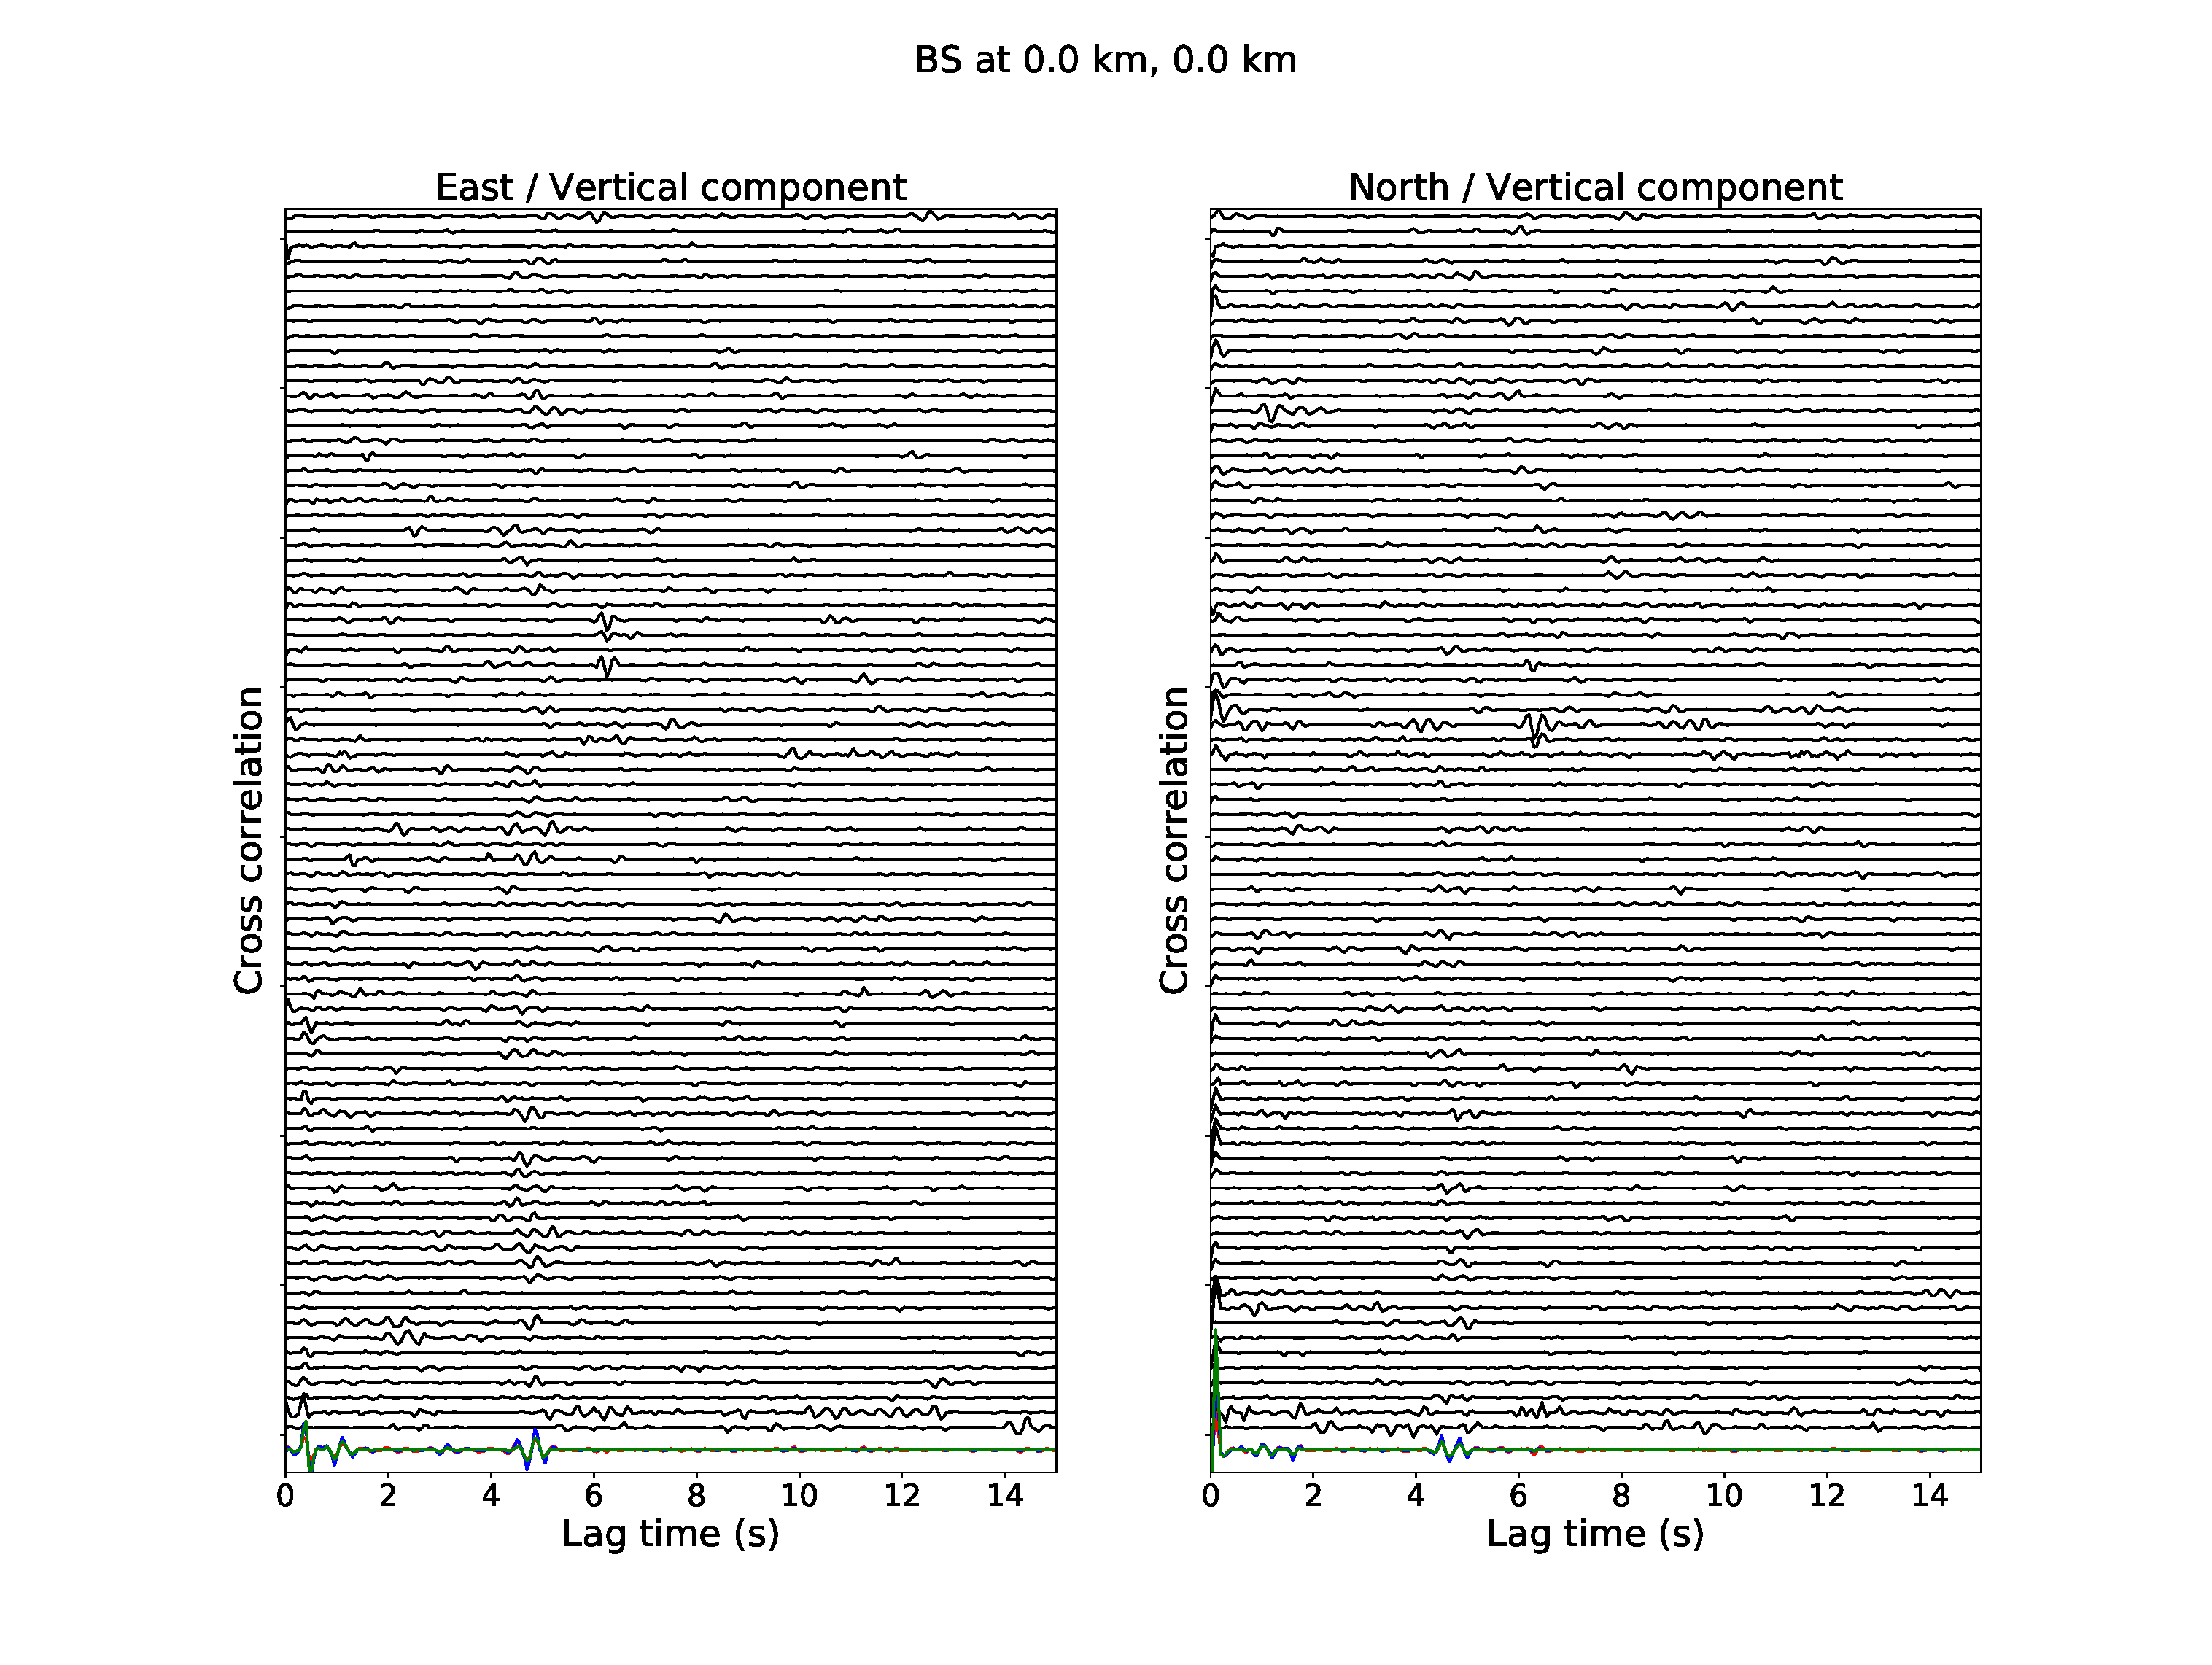
\includegraphics[width=\textwidth, trim={5cm 2cm 5cm 3.5cm},clip]{figures/BS_000_000_PWS.eps}
\caption{Stacked cross correlation functions as function of time for the Big Skidder array for the 82 one-minute long time windows when tremor was detected in a 5 km by 5 km grid cell centered on the array. We used a phase-weighted stack to stack the cross-correlation functions over all the seismic stations. The colored cross-correlation at the end represent the stack over all the 82 time windows, red is for linear-stack, blue is for $n$-root stack and green is for phase-weighted stack. Left panel is the cross correlation of the EW component with the vertical component, and right panel is the cross correlation of the NS component with the vertical component.}
\label{pngfiguresample}
\end{figure}

Only about half of the cross correlation functions have a distinct peak that coincides with the peak in the stacked cross correlation. The other cross correlations functions show either a distinct peak at another time lag, or no clearly visible peak. This may be either because the source of the tremor during the corresponding one-minute-long time window was mislocated, or because the signal-to-noise ratio is too low. To improve the signal-to-noise ratio of the peak in the stacked cross correlation, we divided the one-minute-long time windows into two clusters, the ones that match well the stacked cross correlation, and the ones that do not match it well. For each one-minute-long time window, we computed the maximum absolute value of the cross correlation, its value at time 0, the time at which it takes its maximum absolute value, and the ratio between the
amplitude of the cross correlation peak to the root mean square of the cross correlation function. We did this for both the East-West component and the North-South component. Each one-minute-long time window is thus associated to eight values of quality criteria. We then classified each one-minute-long time window into two different clusters, based on the value of these criteria, using a K-means clustering algorithm (function sklearn.cluster.KMeans from the Python library SciKitLearn). The K-means procedure is as follows: We choose the number of clusters $R$, then we arbitrarily choose a center for each cluster. We put each one-minute-long time window into the cluster to which it is closest (based on the values of the eight criteria). Once all one-minute-long time windows have been put in a cluster, we recompute the mean of the eight criteria for each cluster, and reiterate the procedure until convergence. For each cluster, we then stacked the cross correlation functions over all the one-minute-long time windows belonging to the cluster. Figure 3 shows the envelope of the stacked cross correlation for each of the clusters compared to the original stacked cross correlation for all the one-minute-long time windows. The clustering has improved the amplitude of the peak for one of the clusters, and made the peak nearly disappear for the other cluster.

\begin{figure}
\noindent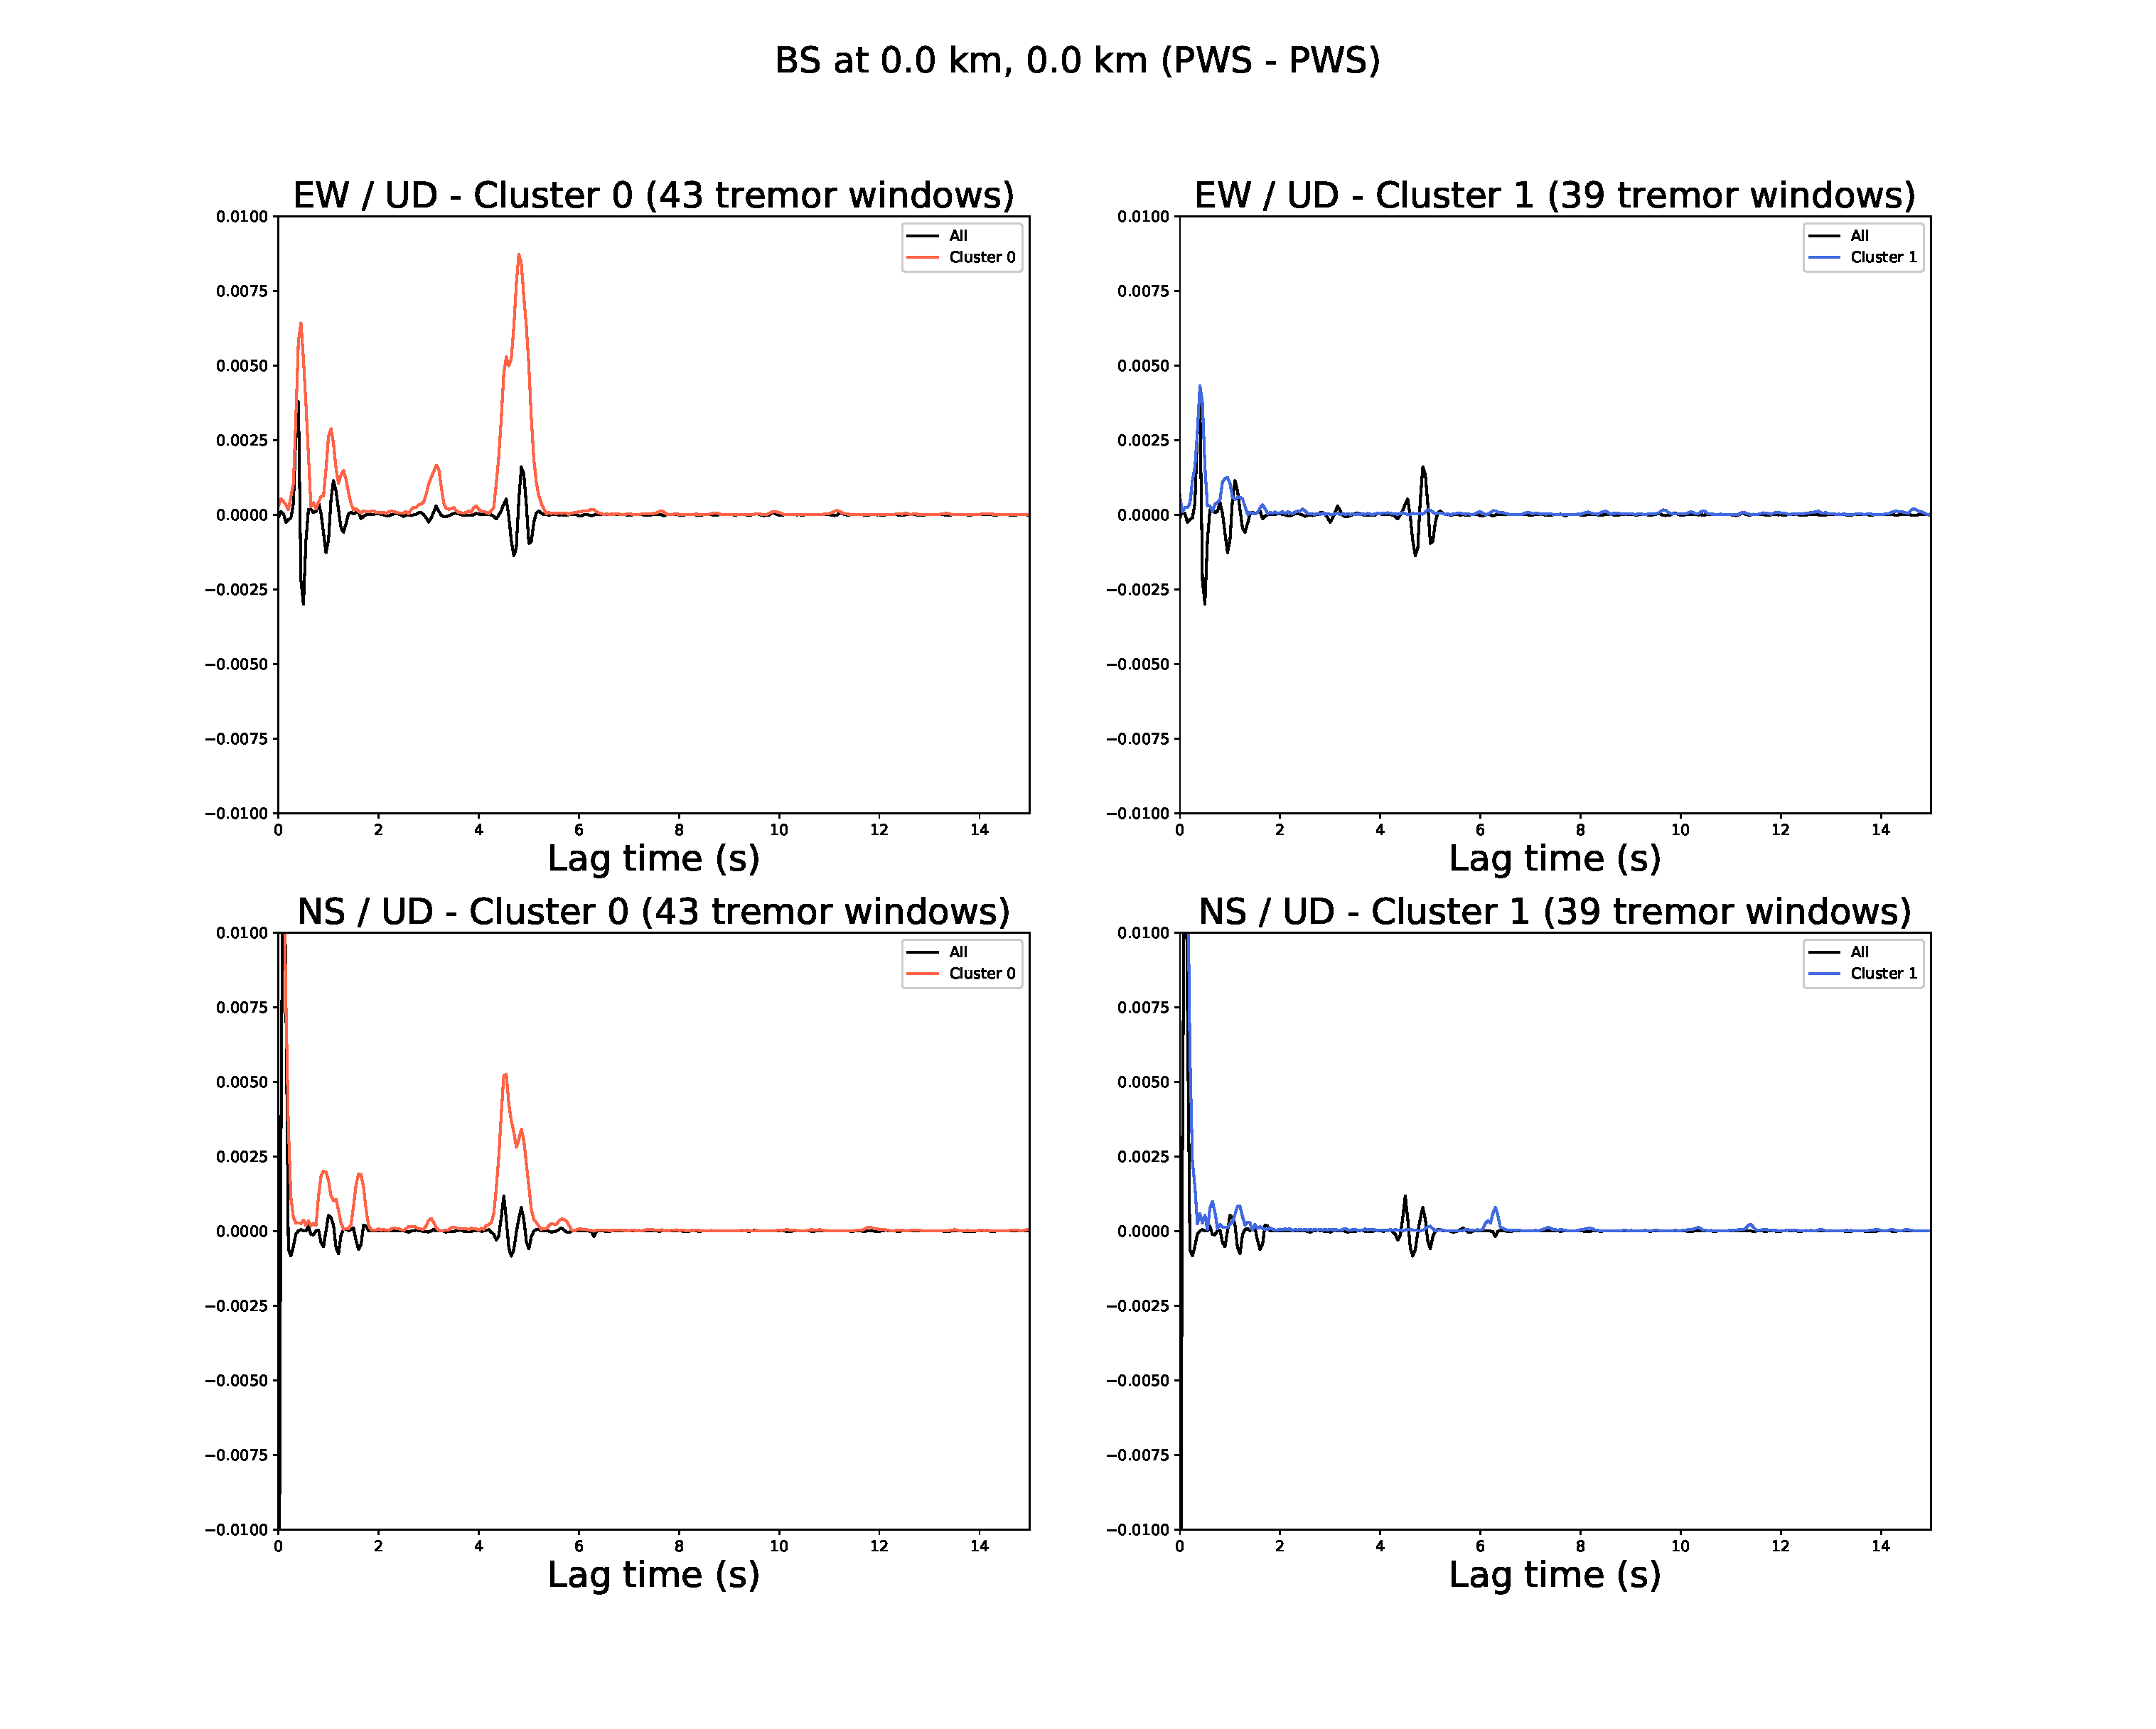
\includegraphics[width=\textwidth, trim={4.5cm 2.5cm 5cm 4cm},clip]{figures/BS_000_000_PWS_PWS_cluster_stackcc.eps}
\caption{Stack of the cross correlation functions over all the 82 time windows from Figure 2. We used a phase-weighted stack for the stack over the stations and for the stack over the time windows. The black line is the stack over all the time windows. The red line on the left panels is the envelope of the stack over the time windows in the first cluster (which contains the time windows that fit well with the stack), and the blue line on the right panels is the envelope of the stack over the time windows in the second cluster (which contains the time windows that do not fit well with the stack). Top panels are the cross correlation of the EW component with the vertical component, and bottom panels are the cross correlation of the NS component with the vertical component.}
\label{pngfiguresample}
\end{figure}

We did this analysis for grid cells located in a 50 km by 50 km area centered on each of the eight arrays. We thus have 11 * 11 * 8 = 968 values of the time lag between the arrival of the direct P-wave and the arrival of the direct S-wave. We first assumed that the source of the tremor is located on the plate boundary, and we took a constant velocity model for the overriding continental crust with $V_P$ = 6.4 km/s and $V_S$ = 3.6 km/s, to compute the depth of the tremor source for each location. % Modify this part if we use a 3D velocity model

\section{Results}

The analysis we carried out above may not lead to a reliable value of the depth of the source of the tremor for all relative positions of the array and the tremor. First, some areas are badly covered, and only a few tremor or no tremor at all were recorded. We limit our analysis to grid cells were tremor has been recorded during at least 10 %to be modified?
one-minute-longtime windows. Second, the method works best for nearly vertical ray paths. A third problem is that we assumed that the location of the tremor source is fixed during the one-minute-long time window where we compute the cross correlation of the seismic signal. However, this is not exactly the case. Indeed, during an ETS event, rapid tremor streaks have been observed propagating in the up-dip and down-dip directions at velocities ranging on average between 30 and 110 km/h ~\cite{GHO_2010_G3}, which corresponds to a maximum source displacement of 0.9 km updip or downdip during the 30 seconds duration before and after the middle of the time window. If we denote $t_P$ the arrival time of the direct P-wave, and $t_S$ the arrival time of the direct S-wave, the time lag between the two phase arrivals is $t_{lag} = t_S - t_P$. During the one-minute time window where we compute the cross correlation, the displacement $dx$ of the tremor source along the plate boundary should corresponds to a time lag difference $dt_{lag}$ shorter than a quarter of the dominant period of the tremor signal $T$ = 0.33 s. We computed the time lag difference for a displacement of the source of 0.9 km in the updip and the downdip directions, for stations aligned along the strike and along the dip direction. We assume that the source was located at 35 km depth, and we look at the time arrivals of the seismic wave for stations located up to 20 km from the epicenter, in the strike or the dip direction. The difference in time lags stays low for all the stations aligned along the strike of the plate boundary. However, for the stations aligned along the dip of the plate boundary, the tremor streaks traveling at 110 km/h will cause a problem for the stations located more than 18 km updip of the tremor source. The difference in time lags stays low for the stations located downdip of the tremor source. \\

\textcolor{red}{Something about how we choose the values we are keeping.} \\

\textcolor{red}{Something about interpolating the values of the different arrays.} \\

\textcolor{red}{Include here Figure 4 of the distance to the plate boundary + include values for the LFE families.} \\

\section{Discussion}

For each of the grid cells and each of the arrays, I will compute the time lag between the direct P-wave and the direct S-wave by taking the maximum value of the envelope of the stacked cross correlation for the cluster containing the time windows that fit best with the stack. I will compare the value of the time lag for the East-West component and the North-South component, to verify whether possible anisotropy in the overriding continental crust introduce a significant difference between both values of the time lag. I will associate an uncertainty to the time lag by computing the width of the envelope at half the amplitude of the maximum. I will then compute the corresponding depth of the tremor, and the associated uncertainty, for each array using a constant velocity model. I will associate to each grid cell and each array a weight related to the ratio between the maximum amplitude of the stack and the root mean square, and interpolate the values of the depth found for the different arrays while taking these weights into account. I will then be able to obtain a map of the depth of the plate boundary, and compare it to the depth of the LFE families identified by ~\citeA{SWE_2019} and ~\citeA{CHE_2017_JGR,CHE_2017_G3}. \\

In the above part, we assumed that all the tremor within a given grid cell originate from the same depth, and we averaged over all the data to get the depth of the tremor source. However, instead of being located on the same plane near the plate boundary, the tremor may be scattered over a layer surrounding the plate boundary. To compute the thickness of this layer, I will compute for each one-minute-long time window for which the cross correlation function matches well the stacked cross correlation the time lag between the time corresponding to the maximum absolute value for the cross correlation function and the time corresponding to the maximum absolute value for the stacked cross correlation. I will then compute the standard deviation of this time lag, and compute the corresponding difference in depth using the constant velocity model that I used previously. %Something about computation of robust standard deviation.
I will thus get the thickness of the layer from which the tremor originate. I will use the same interpolation method as above to get the thickness of the layer for all the area covered by the eight arrays. \\

\textcolor{red}{Some interpretation.}

\section{Conclusion}

%%

%  Numbered lines in equations:
%  To add line numbers to lines in equations,
%  \begin{linenomath*}
%  \begin{equation}
%  \end{equation}
%  \end{linenomath*}



%% Enter Figures and Tables near as possible to where they are first mentioned:
%
% DO NOT USE \psfrag or \subfigure commands.
%
% Figure captions go below the figure.
% Table titles go above tables;  other caption information
%  should be placed in last line of the table, using
% \multicolumn2l{$^a$ This is a table note.}
%
%----------------
% EXAMPLE FIGURE
%
%
% Giving latex a width will help it to scale the figure properly. A simple trick is to use \textwidth. Try this if large figures run off the side of the page.
% \begin{figure}
% \noindent\includegraphics[width=\textwidth]{anothersample.png}
%\caption{caption}
%\label{pngfiguresample}
%\end{figure}
%
%
%
% If you get an error about an unknown bounding box, try specifying the width and height of the figure with the natwidth and natheight options.
% \begin{figure}
% \noindent\includegraphics[natwidth=800px,natheight=600px]{samplefigure.pdf}
%\caption{caption}
%\label{pdffiguresample}
%\end{figure}
%
%
% PDFLatex does not seem to be able to process EPS figures. You may want to try the epstopdf package.
%
%
%
% ---------------
% EXAMPLE TABLE
%
% \begin{table}
% \caption{Time of the Transition Between Phase 1 and Phase 2$^{a}$}
% \centering
% \begin{tabular}{l c}
% \hline
%  Run  & Time (min)  \\
% \hline
%   $l1$  & 260   \\
%   $l2$  & 300   \\
%   $l3$  & 340   \\
%   $h1$  & 270   \\
%   $h2$  & 250   \\
%   $h3$  & 380   \\
%   $r1$  & 370   \\
%   $r2$  & 390   \\
% \hline
% \multicolumn{2}{l}{$^{a}$Footnote text here.}
% \end{tabular}
% \end{table}

%% SIDEWAYS FIGURE and TABLE
% AGU prefers the use of {sidewaystable} over {landscapetable} as it causes fewer problems.
%
% \begin{sidewaysfigure}
% \includegraphics[width=20pc]{figsamp}
% \caption{caption here}
% \label{newfig}
% \end{sidewaysfigure}
%
%  \begin{sidewaystable}
%  \caption{Caption here}
% \label{tab:signif_gap_clos}
%  \begin{tabular}{ccc}
% one&two&three\\
% four&five&six
%  \end{tabular}
%  \end{sidewaystable}

%% If using numbered lines, please surround equations with \begin{linenomath*}...\end{linenomath*}
%\begin{linenomath*}
%\begin{equation}
%y|{f} \sim g(m, \sigma),
%\end{equation}
%\end{linenomath*}

%%% End of body of article

%%%%%%%%%%%%%%%%%%%%%%%%%%%%%%%%
%% Optional Appendix goes here
%
% The \appendix command resets counters and redefines section heads
%
% After typing \appendix
%
%\section{Here Is Appendix Title}
% will show
% A: Here Is Appendix Title
%
%\appendix
%\section{Here is a sample appendix}

%%%%%%%%%%%%%%%%%%%%%%%%%%%%%%%%%%%%%%%%%%%%%%%%%%%%%%%%%%%%%%%%
%
% Optional Glossary, Notation or Acronym section goes here:
%
%%%%%%%%%%%%%%
% Glossary is only allowed in Reviews of Geophysics
%  \begin{glossary}
%  \term{Term}
%   Term Definition here
%  \term{Term}
%   Term Definition here
%  \term{Term}
%   Term Definition here
%  \end{glossary}

%
%%%%%%%%%%%%%%
% Acronyms
%   \begin{acronyms}
%   \acro{Acronym}
%   Definition here
%   \acro{EMOS}
%   Ensemble model output statistics
%   \acro{ECMWF}
%   Centre for Medium-Range Weather Forecasts
%   \end{acronyms}

%
%%%%%%%%%%%%%%
% Notation
%   \begin{notation}
%   \notation{$a+b$} Notation Definition here
%   \notation{$e=mc^2$}
%   Equation in German-born physicist Albert Einstein's theory of special
%  relativity that showed that the increased relativistic mass ($m$) of a
%  body comes from the energy of motion of the body—that is, its kinetic
%  energy ($E$)—divided by the speed of light squared ($c^2$).
%   \end{notation}




%%%%%%%%%%%%%%%%%%%%%%%%%%%%%%%%%%%%%%%%%%%%%%%%%%%%%%%%%%%%%%%%
%
%  ACKNOWLEDGMENTS
%
% The acknowledgments must list:
%
% >>>>	A statement that indicates to the reader where the data
% 	supporting the conclusions can be obtained (for example, in the
% 	references, tables, supporting information, and other databases).
%
% 	All funding sources related to this work from all authors
%
% 	Any real or perceived financial conflicts of interests for any
%	author
%
% 	Other affiliations for any author that may be perceived as
% 	having a conflict of interest with respect to the results of this
% 	paper.
%
%
% It is also the appropriate place to thank colleagues and other contributors.
% AGU does not normally allow dedications.


\acknowledgments
Abhijit Ghosh for catalog. NSF grant number. IGERT Big Data if computations ob AWS.


%% ------------------------------------------------------------------------ %%
%% References and Citations

%%%%%%%%%%%%%%%%%%%%%%%%%%%%%%%%%%%%%%%%%%%%%%%
%
% \bibliography{<name of your .bib file>} don't specify the file extension
%
% don't specify bibliographystyle
%%%%%%%%%%%%%%%%%%%%%%%%%%%%%%%%%%%%%%%%%%%%%%%

\bibliography{bibliography}



%Reference citation instructions and examples:
%
% Please use ONLY \cite and \citeA for reference citations.
% \cite for parenthetical references
% ...as shown in recent studies (Simpson et al., 2019)
% \citeA for in-text citations
% ...Simpson et al. (2019) have shown...
%
%
%...as shown by \citeA{jskilby}.
%...as shown by \citeA{lewin76}, \citeA{carson86}, \citeA{bartoldy02}, and \citeA{rinaldi03}.
%...has been shown \cite{jskilbye}.
%...has been shown \cite{lewin76,carson86,bartoldy02,rinaldi03}.
%...has been shown \cite [e.g.,][]{lewin76,carson86,bartoldy02,rinaldi03}.
%
% DO NOT use other cite commands (e.g., \citet, \citep, \citeyear, \nocite, \citealp, etc.).
%



\end{document}



More Information and Advice:

%% ------------------------------------------------------------------------ %%
%
%  SECTION HEADS
%
%% ------------------------------------------------------------------------ %%

% Capitalize the first letter of each word (except for
% prepositions, conjunctions, and articles that are
% three or fewer letters).

% AGU follows standard outline style; therefore, there cannot be a section 1 without
% a section 2, or a section 2.3.1 without a section 2.3.2.
% Please make sure your section numbers are balanced.
% ---------------
% Level 1 head
%
% Use the \section{} command to identify level 1 heads;
% type the appropriate head wording between the curly
% brackets, as shown below.
%
%An example:
%\section{Level 1 Head: Introduction}
%
% ---------------
% Level 2 head
%
% Use the \subsection{} command to identify level 2 heads.
%An example:
%\subsection{Level 2 Head}
%
% ---------------
% Level 3 head
%
% Use the \subsubsection{} command to identify level 3 heads
%An example:
%\subsubsection{Level 3 Head}
%
%---------------
% Level 4 head
%
% Use the \subsubsubsection{} command to identify level 3 heads
% An example:
%\subsubsubsection{Level 4 Head} An example.
%
%% ------------------------------------------------------------------------ %%
%
%  IN-TEXT LISTS
%
%% ------------------------------------------------------------------------ %%
%
% Do not use bulleted lists; enumerated lists are okay.
% \begin{enumerate}
% \item
% \item
% \item
% \end{enumerate}
%
%% ------------------------------------------------------------------------ %%
%
%  EQUATIONS
%
%% ------------------------------------------------------------------------ %%

% Single-line equations are centered.
% Equation arrays will appear left-aligned.

Math coded inside display math mode \[ ...\]
 will not be numbered, e.g.,:
 \[ x^2=y^2 + z^2\]

 Math coded inside \begin{equation} and \end{equation} will
 be automatically numbered, e.g.,:
 \begin{equation}
 x^2=y^2 + z^2
 \end{equation}


% To create multiline equations, use the
% \begin{eqnarray} and \end{eqnarray} environment
% as demonstrated below.
\begin{eqnarray}
  x_{1} & = & (x - x_{0}) \cos \Theta \nonumber \\
        && + (y - y_{0}) \sin \Theta  \nonumber \\
  y_{1} & = & -(x - x_{0}) \sin \Theta \nonumber \\
        && + (y - y_{0}) \cos \Theta.
\end{eqnarray}

%If you don't want an equation number, use the star form:
%\begin{eqnarray*}...\end{eqnarray*}

% Break each line at a sign of operation
% (+, -, etc.) if possible, with the sign of operation
% on the new line.

% Indent second and subsequent lines to align with
% the first character following the equal sign on the
% first line.

% Use an \hspace{} command to insert horizontal space
% into your equation if necessary. Place an appropriate
% unit of measure between the curly braces, e.g.
% \hspace{1in}; you may have to experiment to achieve
% the correct amount of space.


%% ------------------------------------------------------------------------ %%
%
%  EQUATION NUMBERING: COUNTER
%
%% ------------------------------------------------------------------------ %%

% You may change equation numbering by resetting
% the equation counter or by explicitly numbering
% an equation.

% To explicitly number an equation, type \eqnum{}
% (with the desired number between the brackets)
% after the \begin{equation} or \begin{eqnarray}
% command.  The \eqnum{} command will affect only
% the equation it appears with; LaTeX will number
% any equations appearing later in the manuscript
% according to the equation counter.
%

% If you have a multiline equation that needs only
% one equation number, use a \nonumber command in
% front of the double backslashes (\\) as shown in
% the multiline equation above.

% If you are using line numbers, remember to surround
% equations with \begin{linenomath*}...\end{linenomath*}

%  To add line numbers to lines in equations:
%  \begin{linenomath*}
%  \begin{equation}
%  \end{equation}
%  \end{linenomath*}



